\section{Background}
In this section, we first present the Amdahl's law and performance-per-watt's traditional expression in multi-core processor. Then the static power modeling and thermal modeling is introduced, with which we can revise the expression of performance-per-watt in multi-core processor.




% \subsection{DVFS}


% To find the optimal DVFS frequency that leads to highest energy efficiency, we compare the energy consumption per instruction of each DVFS frequency. Provided Clock cycle Per Instruction (CPI) is one, the energy consumption per instruction (EPI) at frequency $f$ is:
% \begin{equation}
% E = P(f)\cdot \frac{1}{f}
% \end{equation}

% By comparing the energy consumption per instruction of each frequency with the energy consumption per instruction of full frequency, the energy efficiency of each DVFS frequency can be achieved. Note that in real scenerio, the DVFS frequencies are discrete. We set 15 DVFS stages, corresponding to 15 frequencies. For a given processor, the energy efficiency of each DVFS stage can be tested offline. 
% \begin{figure}
% \centering
% \includegraphics[width=1\linewidth]{fig/DVFS.eps}
% \caption{Relative EPI}
% \end{figure}

% As can be seen in Figure. x, the $8^{th}$ DVFS stage is the optimal DVFS stage that leads to highest energy efficiency. The corresponding frequency is $1.95$ GHz. By setting the DVFS stage of each core to the optimal DVFS stage, the energy efficiency of the system is surely the highest. However, the system is also under thermal constraint, sometimes it would violate the thermal limits by setting every core to the optimal DVFS stage. The strategy in this paper is to set the DVFS stage of each core as close to the optimal DVFS stage as possible without violating the thermal constraint.



\subsection{Amdahl's law}
Amdahl's law put an upper bound for the speedup that a multi-core processor can achieve by parallelization as:
\begin{equation}\label{speedup}
Perf = \frac{1} {(1-f)+f/n}
\end{equation}
where $n$ is the number of cores, and $f$ is the fraction of a program's execution time that is parallelizable $(0 \le k \le 1)$. Noted that, (1) is purely theroretical for it doesn't consider any constraints such as power budget.

With the failure of Dennard scaling, Dynamic Voltage and Frequency Scaling (DVFS) has been widely applied in modern processors, which is considered to be an effective technique to achieve trade-off between performance and power consumption. Once a high temperature is detected, DVFS reduces the voltage and frequency of the corresponding core to lower its temperarue. Also DVFS is an effective method to reduce the operating frequency of cores, it's not always true that lower frequency leads to higher energy efficiency, due to the fact that low frequency increases the task execution time.

The DVFS strategy in this paper is to set the DVFS stage of each core as high as possible without violating the thermal constraint.

Considering the performance deterioration introduced by DVFS, we set the ratio of operating frequency with the full frequency as the current core's performance:

\begin{equation}\label{performance_per_core}
D = \frac{F_{o}}{F_{f}},
\end{equation}

Amdahl's law with DVFS can therefore be expressed as:
\begin{equation}\label{speedup}
Perf = \frac{1} {\frac{1-f}{D_{a}}+\frac{f}{\sum_{i=1}^{n}D_{i}}},
\end{equation}
where $D_{a}$ stands for the performance of the active core during sequential computation process, $D_{i}$ stands for the performance of each of the active cores during parallel computation process.

The average power consumption of the many-core processor with DVFS is as follows:
\begin{equation}\label{average_power}
W = \frac{P_{1} \times \frac{1-f}{D_{a}}+P_{n} \times \frac{f}{\sum_{i=1}^{n}D_{i}}}{\frac{1-f}{D_{a}}+\frac{f}{\sum_{i=1}^{n}D_{i}}},
\end{equation}
in which, $P_{1}$ is the power consumption during the sequential computation process, $P_{n}$ is the power consumption during the parallel computation process.

$Perf/W$ of a multi-core processor is expressed as:
\begin{equation}\label{ppw}
\begin{split}
\frac{Perf}{W} &= \frac{1} {\frac{1-f}{D_{a}}+\frac{f}{\sum_{i=1}^{n}D_{i}}} \times \frac{\frac{1-f}{D_{a}}+\frac{f}{\sum_{i=1}^{n}D_{i}}}{P_{1} \times \frac{1-f}{D_{a}}+P_{n} \times \frac{f}{\sum_{i=1}^{n}D_{i}}}\\
&= \frac{1}{P_{1} \times \frac{1-f}{D_{a}}+P_{n} \times \frac{f}{\sum_{i=1}^{n}D_{i}}}
\end{split}
\end{equation}

Likewise, $Perf/J$ of a multi-core processor is expressed as:
\begin{equation}\label{ppw}
\frac{Perf}{J} =\frac{1} {\frac{1-f}{D_{a}}+\frac{f}{\sum_{i=1}^{n}D_{i}}} \times \frac{1}{P_{1} \times \frac{1-f}{D_{a}}+P_{n} \times \frac{f}{\sum_{i=1}^{n}D_{i}}}
\end{equation}

%$P_{1}$ is composed of power consumption of 1 active core and $n-1$ idle cores, if we assume that the power consumption of 1 active core is 1, without consideration of thermal constraints, $P_{1}$ can be expressed as $1+(n-1)k$, in which $k$ stands for the fraction of power the processor consumes in idle state $(0 \le k \le 1)$. For parallel computation phase, $P_{n}$ consists of power consumption of $n$ active cores, which can be similarly expressed as $n$. By replacing $P_{1}$ and $P_{n}$ in (3) with above expressions, we can get
% \begin{equation}\label{ppw}
% \frac{Perf}{W} = \frac{1}{1+k(n-1)(1-f)}
% \end{equation}

% In (4), we ignore the impact of temperature on power consumption of cores, which is 
% With (4) we can plot the relation between performance-per-watt and the number of cores and $f$. 

\subsection{Static power modeling}

It is widely acknowledged that the total power of a chip is composed of dynamic and static power. The dynamic power is dependent on the activities of the chip, therefore it's easily estimated by methods implemented with performance counter. Yet the static power $p_{s}$ of the chip is caused by leakage current $I_{leak}$ as:
\begin{equation}\label{eq:sta_power}
p_{s} = V_{dd}I_{leak}
\end{equation}
Due to the non-linear relationship between $I_{leak}$ and temperature, static power is also sensitive to temperature, which makes it hard to obtain. 

$I_{leak}$ is composed of many components, including subthreshold current, gate current, reverse-biased junction leakage current, et cetera. Among which, subthreshold current and gate current are the main parts of leakage current, therefore $I_{leak}$ can be approximated as:
\begin{equation}\label{eq:leakage}
I_{leak}=I_{sub}+I_{gate}
\end{equation}

Noted that $I_{gate}$ is cause by tunneling between the gate terminal and the other three terminals, does not depend on temperature and can be considered as a technology-dependent constant. Yet $I_{sub}$ is considered to be highly related to temperature, and can be modeled in the commonly accepeted MOSFET transitor model BSIM 4 as:
\begin{equation}\label{eq:sub_current}
I_{sub}=Kv_{T}^{2}e^{\frac{V_{GS}-V_{th}} {\eta v_{T}}} (1-e^{\frac {-V_{DS}} {v_{T}} })\approx Kv_{T}^{2}e^{\frac{V_{GS}-V_{th}}{\eta v_{T}}}
\end{equation}

Apparently, the leakage current has a complex relationship with
temperature. In this work, we use \eqref{eq:sta_power},
\eqref{eq:leakage}, and \eqref{eq:sub_current} to model the static
power considering such relationship. The parameters of
leakage current can be obtained by curve fitting using HSPICE simulation
data. In order to see the accuracy of the model used,
Fig.~\ref{fig:leakage} shows an HSPICE simulation result of leakage using TSMC \SI{65}{nm} process model and its curve fitting result using approximate
leakage model. From the figure, we can see that the static power model
has high accuracy for all common temperatures of IC chips.

\begin{figure}%curve fitting
  \centering
  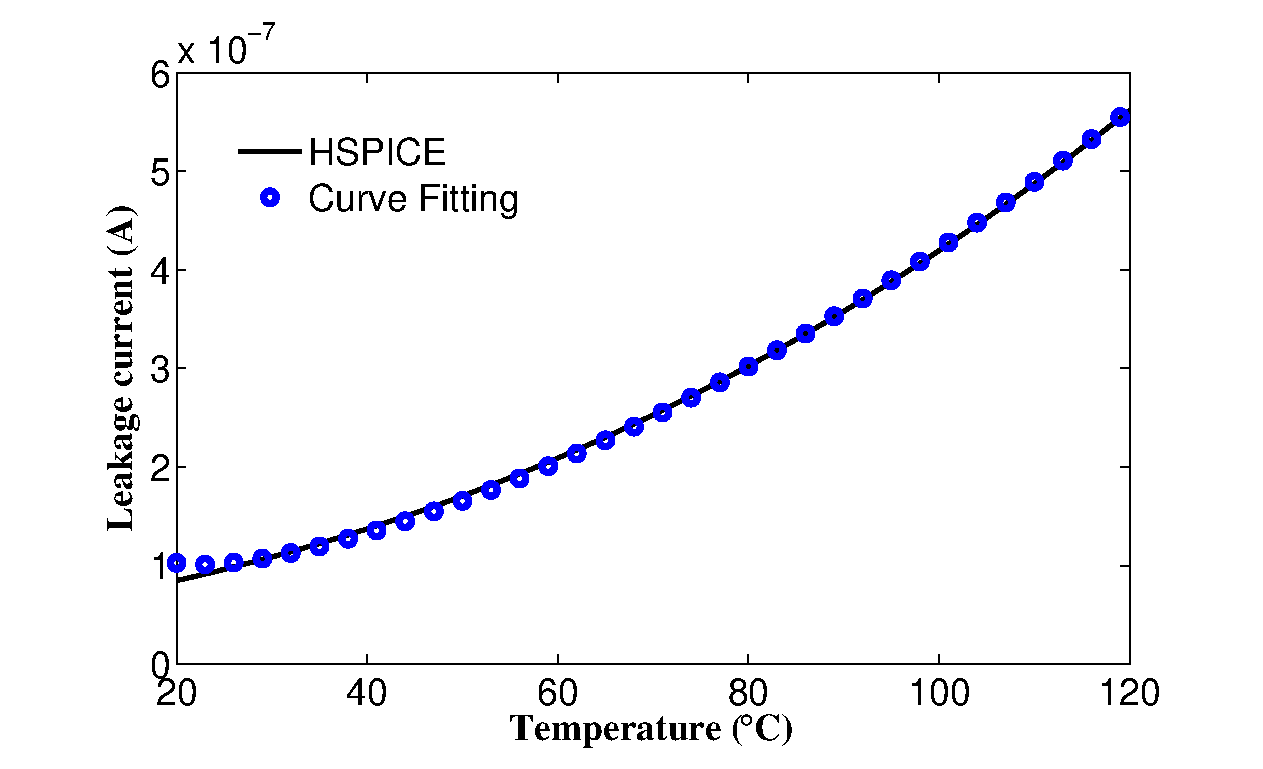
\includegraphics[width=1\columnwidth]{fig/leakage.eps}
  \caption{Comparison of leakage of a TSMC \SI{65}{nm} process MOSFET from HSPICE
    simulation with its curve fitting result using \eqref{eq:sub_current}. An example of
    temperature region division is also shown in the figure, which will be discussed later.}
  \label{fig:leakage}
\end{figure}

We can conclude that the static power distribution depends mainly on
the temperature distribution
for a certain chip with constant physical parameters.
Since temperature also depends on power, in order to view the whole
picture, thermal model of IC chip is used to describe
temperature's dependency on power as shown next.


\subsection{Thermal modeling}
In this work, the multi-core dark silicon system is packaged in a common structure in Fig. x. 
To estimate the power consumption of a IC chip, we first divide the chip and its package into multiple blocks called thermal nodes, with partition granularity determined by the accuracy requirements. For the dark silicon multi-core system (a 16-core chip's floorplan example is shown in Fig. x), we treat each core as a thermal node with a current source, because each core has very small area and highly correlated internal power distribution. The other thermal nodes from the package are divided according to the chip thermal nodes. Then, the thermal resistance and capacitance among these thermal nodes are determinded, which model the thermal transport and power response behaviors. Please note that multi-core system floorplan different from the one shown in Fig. x are fullly compatible with this work, and each core's internal structure can also be modeled if necessary. With above mentioned information, the thermal mdoel for a chip with $n$ total thermal nodes can be generated:
\begin{equation}\label{gt=bp}
\begin{split}
GT(t) + C\frac{dT(t)}{dt} &= BP_{T}\\
T_{c}(t) &= LT_{t}
\end{split}
\end{equation}
where $T(t) \in \mathbb{R}^n$ is the temperature vector (distinguished from $T_p$, which is a scalar representing temperature at only one place), representing temperatures at $n$ places of the chip and package; $G \in \mathbb{R}^{n\times n}$ and  $C \in \mathbb{R}^{n \times n}$ contain equivalent thermal resistance and capacitance information respectively; $B \in \mathbb{R}^{n \times l}$ stores the information of how powers are injected into the thermal nodes; $P(T, t) \in \mathbb{R}^{l}$ is the power vector, which contains power consumptions of $l$ components on chip, including both dynamic power vector $P_d$ and static power vector $P_s$, i.e., $P(T, t)=P_s(T, t)+P_d(t)$, reminding that static power $P_s(T, t)$ is actually a function of temperature $T$;  $T_{c}(t) \in \mathbb{R}^m$ is the output temperature vector, containing only temperatures of thermal nodes that the user is interested in, for example, thermal nodes on the chip only (excluding package thermal nodes); $L \in \mathbb{R}^{m \times n}$ is the corresponding output selection matrix which selects the $m$ chip temperatures from $T(t)$.

By applying thermal model, the effect of temperature on cores can be introduced. Through appropriate search methods, the number and distribution of light core with the maximum PPW for number of light cores from $1$ to $n$ can be specified.



